\documentclass[10pt,a4paper]{book}
\usepackage[utf8]{inputenc}
\usepackage[T1]{fontenc}
\usepackage{amsmath}
\usepackage{amsthm}
\usepackage{ctex}
\usepackage{amsfonts}
\usepackage{amssymb}
\usepackage{graphicx}

\usepackage{listings}   % include the package before using it

\newtheorem{theorem}{Theorem}[section]
\newtheorem{lemma}{Lemma}[section]
\newtheorem{corollary}{Corollary}[section]

%//LaTeX 头部添加
%\newtheorem{theorem}{Theorem}[section]
%
%\begin{theorem}
%	***//定理内容
%	\label{thm-1}
%\end{theorem}
%
%\begin{proof}
%	***//证明过程
%\end{proof}
%
%//LaTeX 头部添加
%\newtheorem{lemma}{Lemma}[section]
%
%\begin{lemma} 
%	***//引理内容
%	\label{lem-1}
%\end{lemma}
%
%//LaTeX 头部添加
%\newtheorem{corollary}{Corollary}[section]
%
%\begin{corollary} 
%	***//推论内容
%	\label{cor-1}
%\end{corollary}



\begin{document}
	\chapter{2020年笔记}
	\section{20.07.27}
	\begin{equation}
		\begin{aligned}
			I &= \int_{\frac{\pi}{4}}^{\pi}\int_{0}^{2\sin\theta} f(r\cos\theta,r\sin\theta)r\text{d}r\text{d}\theta\\	
			&=[\int_{0}^{\sqrt{2}}\int_{\frac{\pi}{4}}^{\pi-\arcsin\frac{r}{2}} 
			+ \int_{\sqrt{2}}^{2} \int_{\arcsin\frac{r}{2}}^{\pi-\arcsin\frac{r}{2}}  ]
			f(r\cos\theta,r\sin\theta)r\text{d}r\text{d}\theta\\
		\end{aligned}
	\end{equation}
	
	\section{20.08.03}
	
	\begin{equation}
		\lim\limits_{n \rightarrow +\infty }
	(1-\frac{1}{1+2})(1-\frac{1}{1+2}) (1-\frac{1}{1+2+3})\dots(1-\frac{1}{1+2+\dots+n}) = ?
	\end{equation}

	\begin{equation}
		\begin{aligned}
			1-\frac{1}{\frac{n(n+1)}{2}} &= 1-\frac{2}{n(n+1)}\\
			&=\frac{n^2+n-2}{n(n+1)}\\
			&=\frac{(n+2)(n-1)}{n(n+1)}
		\end{aligned}
	\end{equation}
	
	\begin{equation}
		\begin{aligned}
			I&=\lim\limits_{n\rightarrow +\infty}\frac{1\times 4}{2\times 3}\frac{2\times 5}{3\times 4}\dots \frac{(n-2)(n+1)}{(n-1)n}\frac{(n-1)(n+2)}{n(n+1)}\\
			&=\lim\limits_{n\rightarrow+\infty}\frac{1}{3}\frac{4}{2}\frac{2}{4}\frac{5}{3}\frac{3}{5}\frac{6}{4}\dots \frac{n+2}{n}\\
			&=\lim\limits_{n\rightarrow+\infty}\frac{1}{3}\frac{n+2}{n}\\
			&=\frac{1}{3}\lim\limits_{n \rightarrow +\infty }\frac{n+2}{n}\\
			&=\frac{1}{3}
		\end{aligned}
	\end{equation}
	\\
	\\
	\\
	卡塔兰数 $ C_n $
	
	从0开始 $ 1, 1, 2, 5, 14, 42, \dots $
	\[
	C_{n+1} = C_0 C_n + C_1 C_{n-1} + \dots + C_n C_0
	\]
	
	该公式的证明可以通过
	\[
	\Bigg( \bigg( \Big( \big( \Bigg) \bigg) \Big) \big)
	\]
	如图所示的括号匹配,$ C_n $可以看成上面四组括号的合理排列形式,(合理排列意味着每一对括号都是左右对应的,像$ )( $这样的形式是非法的)
	
	在$ n $对括号的排列中,假设最后一个括号和第$ i $个左括号匹配。则在第$ i $个左括号之前,一定已经匹配上了$ (i-1) $对左括号。如下图,因此,此种情况的数量为$ f(i-1)*f(n-i-1) $。$ (1\leq i\leq n) $最后一个右括号可以$ 1 \sim n $个左括号匹配共n种情况。
	
	\begin{figure} [h]
		\centering
		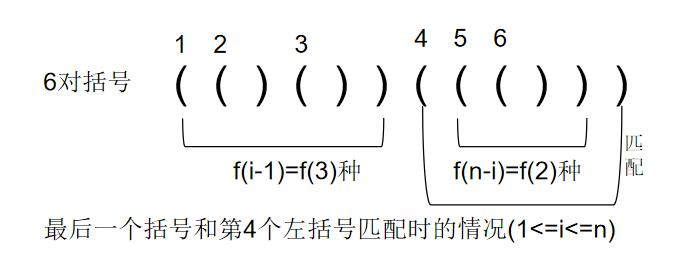
\includegraphics[width=0.7\linewidth]{pic/catalan_proof-001}
		\caption{catalan number - proof}
		\label{fig:catalanproof-001}
	\end{figure}
	
	
%	\[
%???	(n-3)C_n = \frac{n}{2}(C_3 C_{n-1} + C_4 C_{n-2} + \dots + C_{n-2} C_4 + C_{n-1} C_3 )
%	\]
	第$ n+1 $项 
	\[C(n) = \frac{C^n_{2n}}{n+1} \]
	\[	C(n) = C_{2n}^n-C_{2n}^{n-1} = \frac{C_{2n}^n}{n+1}	\]
	
	通项公式
	\[ C_1 = 1, C_n = C_{n-1}\frac{4n-2}{n+1} \]
	
	
	Python 实现
	
	
	\begin{lstlisting}[language=Python]
		# 打印前 n 个卡特兰数
		ans, n = 1, 20
		print("1:" + str(ans))
		for i in range(2, n + 1):
		ans = ans * (4 * i - 2) // (i + 1)
		print(str(i) + ":" + str(ans))
	\end{lstlisting}
	
	
	扩展\\
	
	最后留一道比较有意思的卡特兰数问题,欢迎读者留言,提出自己的看法。
	
	8 个高矮不同的人需要排成两队,每队 4 个人。其中,每排都是从低到高排列,且第二排的第 i 个人比第一排中第 i 个人高,则有多少种排队方式。
	
	
	
	\section{20.08.07}
	

	
	
	
	\begin{theorem}
	A-G 不等式\\ 任意n个非负实数$ a_1, a_2, \dots, a_n$ \\
	\begin{equation}
		\frac{a_1 + a_2 + \dots + a_n}{n} \geq \sqrt[n]{a_1\dots a_n}
	\end{equation}
	其中等号成立 $\iff a_1 = a_2 = \dots = a_n$

	\label{thm-1}
	\end{theorem}

	\begin{proof}\label{1}
	数学归纳法\\ $n=1$时结论平凡\\
	$n=2\qquad \frac{a_1+a_2}{2} \geq \sqrt{a_1a_2}$\\
	\[(a_1 - a_2)^2 = a_1^2 - 2 a_1 a_2 + a_2^2 \geq 0 \]
	\[a_1^2 + 2a_1a_2 + a_2^2 \geq 4a_1a_2\]
	\[(a_1+a_2)^2\geq 4a_1a_2\]
	\[\frac{a_1+a_2}{2}\geq \sqrt{a_1a_2}\]
	$n=k$时,假设 $\frac{a_1+\dots+a_k}{k}\geq \sqrt[k]{a_1\dots a_k}$成立\\
	$ n=k+1 $
	\begin{equation}
	\begin{aligned}
		&\frac{a_1+\dots + a_k + a_{k+1}}{k+1}-\frac{a_1+\dots +a_k}{k} \\
		=&\frac{k(a_1+\dots+a_{k+1})-(k+1)(a_1+\dots+a_k)}{k(k+1)}\\
		=&\frac{ka_{k+1}-(a_1+\dots+a_k)}{k(k+1)}\\		
	\end{aligned}
	\end{equation}
	we found 
	\[\frac{a_1+\dots + a_k + a_{k+1}}{k+1} =  \frac{a_1+\dots + a_k}{k} + \frac{ka_{k+1}-(a_1+\dots + a_k)}{k(k+1)} \]
	note \[ A := \frac{a_1+\dots + a_k}{k} , \qquad B:=\frac{ka_{k+1}-(a_1+\dots + a_k)}{k(k+1)}\]
	
	\begin{equation}
		(\frac{a_1+\dots + a_k + a_{k+1}}{k+1})^{k+1}=(A+B)^{k+1}\geq A^{k+1}+(k+1)A^k B
	\end{equation}
	使用二项式展开需要对$ a_i $从小到大重排,而使用Bernoulli不等式则只需要$ A\geq 0, (A+B)\geq 0 $即可
	\begin{equation}
		A^{k+1}+(k+1)A^k B = A^k(A+(k+1)B)
	\end{equation}
	\begin{equation}
		\begin{aligned}
			A^k& =	(\frac{a_1+\dots + a_k + a_{k+1}}{k+1})^{k+1} \geq a_1\dots a_k \quad \text{assume at}(n=k)\\
			A+(k+1)B&= \frac{a_1+\dots + a_k}{k} + \frac{ka_{k+1}-(a_1+\dots + a_k)}{k} = a_{k+1}\\
			\because& (A+B)^{k+1}\geq A^k(A+(k+1)B)\geq a_1 \dots a_k  a_{k+1}\\
			\therefore & 	\frac{a_1+\dots + a_k + a_{k+1}}{k+1} \geq  \sqrt[k+1]{a_1 \dots a_k  a_{k+1}}\\
		\end{aligned}
	\end{equation}
	
	使用二项式展开定理的条件:\\
	在归纳法第二步对$a_1 \dots a_{k+1}  $重编号,使$ a_{k+1} $为其中最大的数(之一)\\
	这使得分解式右边第二项$ \frac{ka_{k+1}-(a_1+\dots+a_k)}{k(k+1)} $ 一定是非负数
	\end{proof}
	
	
	\begin{proof}\label{证明 2}
	Forward and backward (Cauchy, 1897)\\
	Forward Part:\\
	$ n=2 $ 
	\begin{equation}
		\frac{a_1+a_2}{2}\geq \sqrt{a_1a_2}
	\end{equation}
	$ n=4 $ 
	\begin{equation}
		\begin{aligned}
			\frac{a_1+a_2+a_3+a_4}{4}
			&\geq \sqrt{\frac{a_1+a_2}{2}\frac{a_3+a_4}{2}}\\
			&\geq \sqrt{\sqrt{a_1a_2}\sqrt{a_3a_4}}\\
			&\geq \sqrt[4]{a_1a_2a_3a_4}\\
		\end{aligned}
	\end{equation}
	$ n=2^k $ 假设不等式$ \frac{a_1+\dots +a_{2^k}}{2^k}\geq \sqrt[2^k]{a_1\dots a_{2^k}} $成立\\
	$ n=2^{k+1} $
	\begin{equation}
		\begin{aligned}
			\frac{a_1+\dots+a_{2^k}+\dots+a_{2^{k+1}}}{2^{k+1}}
			&\geq \sqrt{\frac{a_1+\dots +a_{2^k}}{2^k}\frac{a_{2^k+1}+\dots +a_{2^{k+1}}}{2^k}}\\
			&\geq \sqrt{\sqrt[2^k]{a_1\dots a_{2^k}}\sqrt[2^k]{a_{2^k+1}\dots a_{2^{k+1}}}}\\
			&\geq \sqrt[2^{k+1}]{a_1\dots a_{2^{k+1}}}
		\end{aligned}
	\end{equation}
	
	Backward Part:
	A-G不等式对某个$ n\geq 2 $成立,则它对$ n-1 $也成立
	\begin{equation}
		\begin{aligned}
			\frac{1}{n-1}\sum_{i=1}^{n-1}a_i 
			&= \frac{1}{n}(\frac{n}{n-1})\sum_{i=1}^{n-1}a_i\\
			&=\frac{1}{n}(\sum_{i=1}^{n-1}a_i+\frac{1}{n-1}\sum_{i=1}^{n-1}a_i)
		\end{aligned}
	\end{equation}
	将$ \frac{1}{n-1}\sum_{i=1}^{n-1}a_i $看作$ a_n $
	\begin{equation}
		\frac{1}{n-1}\sum_{i=1}^{n-1}a_i
		\geq \sqrt[n]{(\prod_{i=1}^{n-1}a_i) (\frac{1}{n-1}\sum_{i=1}^{n-1}a_i)}
	\end{equation}
	
	\begin{equation}	
		(\frac{1}{n-1}\sum_{i=1}^{n-1}a_i)^n
		\geq \prod_{i=1}^{n-1}a_i(\frac{1}{n-1}\sum_{i=1}^{n-1}a_i)
	\end{equation}
	

	\begin{equation}	
		(\frac{1}{n-1}\sum_{i=1}^{n-1}a_i)^{n-1}
		\geq \prod_{i=1}^{n-1}a_i
	\end{equation}


	\begin{equation}		
		\frac{1}{n-1}\sum_{i=1}^{n-1}a_i
		\geq \sqrt[n-1]{\prod_{i=1}^{n-1}a_i}
	\end{equation}


	\begin{equation}
		\frac{1}{n-1}\sum_{i=1}^{n-1}a_i \geq \sqrt[n]{(\prod_{i=1}^{n-1}a_i)(\frac{1}{n-1}\sum_{i=1}^{n-1}a_i)}
	\end{equation}
	
	\begin{equation}
		( \frac{1}{n-1}\sum_{i=1}^{n-1}a_i )^n \geq \prod_{i=1}^{n-1}a_i(\frac{1}{n-1}\sum_{i=1}^{n-1}a_i)
	\end{equation}

	\begin{equation}
		( \frac{1}{n-1}\sum_{i=1}^{n-1}a_i )^{n-1} \geq \prod_{i=1}^{n-1}a_i
	\end{equation}
	
	\begin{equation}
		 \frac{1}{n-1}\sum_{i=1}^{n-1}a_i  \geq \sqrt[n-1]{\prod_{i=1}^{n-1}a_i}
	\end{equation}
	
	\end{proof}
	
	\begin{theorem}
		柯西,施瓦茨不等式\\	
		对$ a_1,\dots,a_n $和$ b_1, \dots ,b_n \in \mathbb{R}$,成立
		\begin{equation}
			|\sum_{i=1}^n a_ib_i|\leq \sqrt{\sum_{i=1}^n a_i^2}\sqrt{\sum_{i=1}^n b_i^2}
		\end{equation}
		\label{1.3.5}
	\end{theorem}
	


	\section{20.08.12}
	1.3.2 练习题
	
	1. (1) 伯努利不等式推广\\solve:
	\[ -2 \leq h \leq -1 \]
	\[ -1 \leq 1+h \leq 0 \]
	\[ -1 \leq (1+h)^n \leq 0 \]
	\[ -2n \leq nh \leq -n \]
	\[ 1-2n \leq 1+nh \leq 1-n \]
	
	$ n=0 \qquad (1+h)^0 = 1 = 1+0*h $  结果是平凡的
	
	$ n=1 \qquad 1+h = 1+h $ 结果是平凡的
	
	$ n \geq 2 \qquad $ 此时 $ 1-n \leq -2 $
	\[ 0 \geq (1+h)^n \geq -1 \geq -2 \geq 1-n \geq 1-nh \geq 1- 2n  \]
	\[ (1+h)^n \geq 1+nh \]
	
	1. (2)
	$ h\geq 0 \qquad (1+h)^n \geq \frac{n(n-1)h^2}{2}$ 
	\[ (1+h)^n=1+nh+\frac{n(n-1)}{2}h^2 + \dots \geq \frac{n(n-1)}{2}h^2  \]
	
	推广:
	\[ (1+h)^n \geq C_n^3 h^3, C_n^4 h^4, \dots , C_n^k h^k ,\qquad 0\leq k\leq n\]
	1. (3)
	$ a_i \ge -1 $且同号
	(a)$ a_i \ge 0$, 且同号。$ \prod(1+a_i) $ 
	
	
\end{document}